\subsection{Problemas en el Desarrollo}
\label{subsec:desarrollo-problemas}

En esta sección se detallarán algunos de los problemas que se fueron teniendo a lo largo del TP y cómo se solucionaron.

\subsection{Intercalar sonido original con efecto}
\label{subsec:desarrollo-problemas-stereo-output}
Luego de la recomendación de separar el audio original y el efecto en los distintos canales (\ref{output-stereo}), se me dificultó saber cómo hacerlo. El problema provenía de no saber cómo hacer para intercalar las muestras correspondientes a los distintos canales, si no era serializando (haciendo sobre cada muestra por separado, poniéndolas en algún registro xmm, y después shuffleando para seguir con la muestra siguiente) las operaciones. 

Analizando el set de instrucciones disponibles, se encontraron \textbf{punpckchdq} y \textbf{punpckcldq} que permiten intercalar los valores ``altos'' o ``bajos'' (respectivamente) de dos registros xmm distintos. Teniendo un registro con la señal original y otro con la señal húmeda, se puede lograr justamente lo que se quería. \vspace{\baselineskip}

\fbox{\begin{minipage}{42em}
\underline{Nota}: si bien las figuras \ref{fig:punpckhdq} y \ref{fig:punpckldq} tienen 64 bits, las instrucciones operan en x64 sobre los registros xmm enteros, de 128 bits.
\end{minipage}}

\begin{figure}[H]
    \centering
    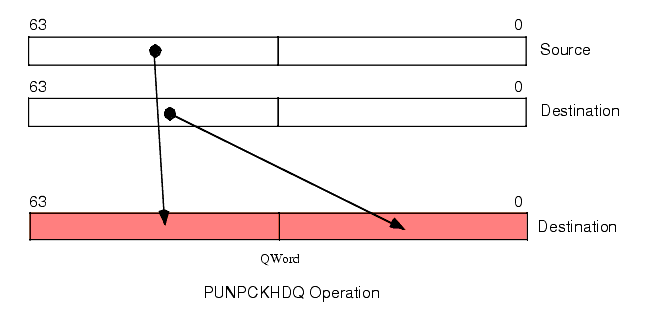
\includegraphics[scale=0.75]{imagenes/punpckhdq.png}
    \label{fig:punpckhdq}
    \caption{}
\end{figure}

\begin{figure}[H]
    \centering
    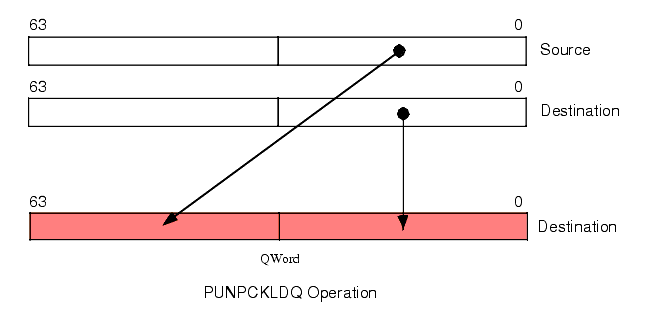
\includegraphics[scale=0.75]{imagenes/punpckldq.png}
    \label{fig:punpckldq}
    \caption{}
\end{figure}

\subsection{Seno}
\label{subsec:desarrollo-problemas-seno}
En las primeras versiones finales de algunos efectos (flanger, wahwah, vibrato), se utilizó la librería \fullref{subsec:ssemath} para poder utilizar el seno sobre un vector de valores. Sin embargo, el análisis de rendimiento mediante la librería \textbf{Tiempo.h} reveló que los efectos en Assembler eran considerablemente más lentos que los de C, aunque las razones no eran claras. Se realizó entonces un análisis mediante una herramienta de profiling, \fullref{subsec:callgrind}. Los resultados de este análisis se ven en las siguientes imágenes:

\begin{figure}[H]
    \centering
    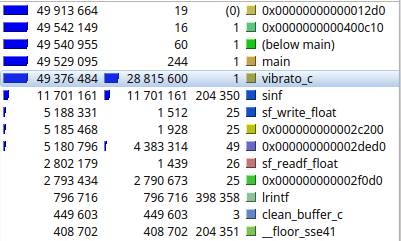
\includegraphics[scale=0.8]{imagenes/callgrind-c.png}
    \label{fig:callgrind-c-26787}
    \caption{Efecto Vibrato en C, argumentos 0.001 y 4.3}
\end{figure}

\begin{figure}[H]
    \centering
    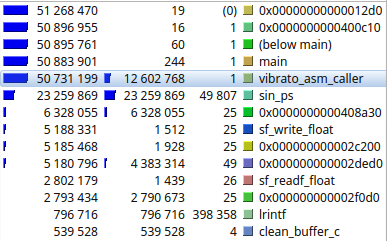
\includegraphics[scale=0.8]{imagenes/callgrind-asm.png}
    \label{fig:callgrind-asm-26788}
    \caption{Efecto Vibrato en ASM, argumentos 0.001 y 4.3}
\end{figure}

En las figuras anteriores, la primera columna indica el costo de la función que fue llamada (tercera columna) sumado al costo de sus hijos, la segunda columna únicamente el costo de esa función (sin el de los hijos), y la tercera columna cuántas veces fue llamada la función. Se puede observar que \textbf{C} y \textbf{Assembler} poseen un costo similar en total (cerca de los 50.000.000), y que este último tiene un costo bastante alto para la operación correspondiente al seno calculado con la librería \textbf{ssemath} (\textit{sin\_ps}).

Utilizando la rutina alternativa para el seno (\ref{subsec:desarrollo-seno}) en \textbf{ASM}, el resultado es el siguiente:

\begin{figure}[H]
    \centering
    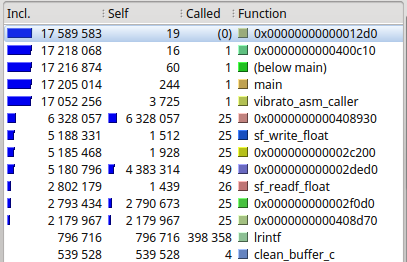
\includegraphics[scale=0.8]{imagenes/callgrind-asm-seno-approx.png}
    \label{fig:callgrind-asm-27462}
    \caption{Efecto Vibrato (seno aproximado) en ASM, argumentos 0.001 y 4.3}
\end{figure}

Se puede ver que se logró el efecto buscado: se redujo el costo de aplicar el efecto en \textbf{ASM} muy por debajo de su contraparte en \textbf{C}. Si bien resulta injusto comparar un seno aproximado con el provisto por la librería \textbf{math.h}, utilizar la rutina aproximada en \textbf{C} no da buenos resultados:

\begin{figure}[H]
    \centering
    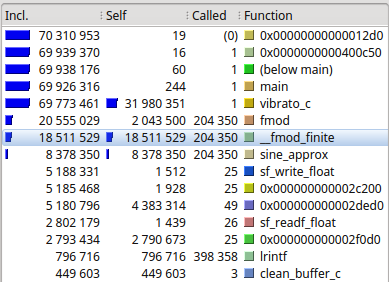
\includegraphics[scale=0.8]{imagenes/callgrind-c-seno-approx.png}
    \label{fig:callgrind-asm-27512}
    \caption{Efecto Vibrato (seno aproximado) en C, argumentos 0.001 y 4.3}
\end{figure}


\subsection{Restas versus división}
\label{subsec:desarrollo-problemas-modulo}
Uno de los requerimientos de la rutina del seno aproximado es que el argumento de la función se debe encontrar entre $(-\pi,\pi)$. Como se puede ver, eso lleva a que en la figura \ref{fig:callgrind-asm-27512} tenga un alto costo lo concerniente a la operación módulo. 

En un principio, para el código en \textbf{ASM}, se llevaban los argumentos del seno al rango mencionado mediante restas. Sin embargo, como los argumentos podían estar bastante lejos del intervalo $(-\pi, \pi)$ (pues dependen del índice de la muestra, que puede ser un número muy grande aún en archivos de algunos pocos segundos), el número de saltos que se hacían en el siguiente pedazo de código perjudicaba bastante el rendimiento:\vspace{\baselineskip}

\lstset{language=[x86masm]Assembler}
\begin{lstlisting}[frame=single]
  arg_to_interval:
        movaps cmpflag, pi              
	  ; cmpflag = |pi|pi|pi|pi|
        cmpps cmpflag, sine_args, 0x01  
	  ; cmpflag = pi < sine_args
        ptest cmpflag, cmpflag
        jz calc_sine    ; 0 => no hay ningún argumento mayor que pi

        movaps tmp, two_pi
        andps tmp, cmpflag              
	  ; me quedo con 2*pi en los lugares donde pi < sine_args
        subps sine_args, tmp            
	  ; resto -2*pi en los lugares que corresponden

        jmp arg_to_interval
\end{lstlisting}

El cálculo del módulo mediante restas se debía a la aversión a utilizar la división, por ser muy costosa generalmente. Sin embargo, en este caso se terminó optando por dividir, quedarse con la parte entera de la división, multiplicar por el divisor, y restar este resultado al valor original, para realizar la operación de módulo. Esta solución probó ser mucho más rápida que la que utilizaba restas, al no tener tantos saltos como el código anteriormente citado.

\subsection{Normalización}
\label{subsec:desarrollo-problemas-normalizacion}

En la aplicación del efecto \fullref{subsec:desarrollo-wahwah}, era posible que la señal húmeda final se encontrara saturada por las operaciones realizadas. Fue necesario entonces realizar la normalización del archivo, comprometiendo un poco la \textit{fidelidad} del efecto, pero entre varias alternativas consideradas fue la más apropiada.

Una opción era realizar una normalización por completo del canal \textit{húmedo} del archivo, luego de la aplicación del efecto. Esta solución no era viable, puesto que el canal ya se encontraba saturado en algunas secciones, y el ruido generado por ese defecto se seguía sintiendo aún después de la normalización.

Otra opción considerada fue realizar normalizaciones ``parciales'' por cada ciclo de lectura del archivo original. Es decir, leer una sección del archivo de audio original, aplicar el efecto, y normalizar únicamente esta porción de la señal. Debido a la gran diferencia entre una sección de la señal y otras, esto generaba una gran deformación de la señal húmeda, ya que existía un máximo absoluto en cada ciclo, algo que por las características en general de una señal de audio no suele suceder.

Finalmente, se terminó multiplicando la señal húmeda final por un modificador arbitrario, \textit{0.1}, para disminuir la amplitud de la señal, y luego normalizar el archivo entero. Si bien no es lo más óptimo en cuanto a rendimiento (se recorre el archivo entero tres veces: una para aplicar el fecto, otra para encontrar el máximo valor de la señal húmeda, y una tercera para normalizar), es la solución que terminó otorgando la mejor calidad de sonido posible, sin distorsiones auditivas.